%\documentclass[tikz,convert={outfile=\s1.svg}]{standalone}
\documentclass[tikz]{standalone}
\usepackage{amsthm}
\usepackage[landscape]{geometry}
\usepackage{multicol}
\usepackage{tikz}
\usepackage{pgfplots}
\usepackage{xcolor}
\usepackage{amsmath}
\usepackage[T1]{fontenc}
\usepackage{utopia}
\usepackage{changepage}
\usepackage{amssymb}
\usepackage{fancyhdr}
\usepackage[many]{tcolorbox}
\usepackage{moresize}
\usepackage{fullpage}
\usepackage{mathpazo}
\usepackage{tikz-3dplot}
\usepackage{cancel}
\tdplotsetmaincoords{70}{165}
\pgfplotsset{compat=1.18}
\usepackage{enumitem}
\usepackage{tabularray}
\usepackage{mathtools}

\UseTblrLibrary{diagbox}

\usetikzlibrary{
    shadings, calc, patterns, angles, quotes, arrows.meta, 
    decorations.pathmorphing, decorations.pathreplacing, 
    fadings, 3d, perspective, backgrounds, intersections, 
    decorations.markings, bending, positioning, 							spy,shapes.geometric,shadows,shapes.symbols, fadings, matrix, fit
}

\usepgfplotslibrary{
    groupplots, external, colormaps, patchplots, fillbetween
}


% Reds (r)
\definecolor{r1}{RGB}{255, 191, 191}    % Light coral
\definecolor{r2}{RGB}{255, 191, 223}    % Light pink
\definecolor{r3}{RGB}{255, 207, 207}    % Light rose

% Blues (b)
\definecolor{b1}{RGB}{191, 223, 255}    % Light blue
\definecolor{b2}{RGB}{191, 239, 255}    % Light sky
\definecolor{b3}{RGB}{191, 255, 255}    % Light cyan

% Greens (g)
\definecolor{g1}{RGB}{191, 255, 191}    % Light green
\definecolor{g2}{RGB}{191, 255, 223}    % Light mint
\definecolor{g3}{RGB}{207, 255, 207}    % Light sage

% Oranges (o)
\definecolor{o1}{RGB}{255, 223, 191}    % Light peach
\definecolor{o2}{RGB}{255, 239, 191}    % Light cream
\definecolor{o3}{RGB}{255, 231, 191}    % Light buff

% Violets (v)
\definecolor{v1}{RGB}{223, 191, 255}    % Light purple
\definecolor{v2}{RGB}{239, 191, 255}    % Light lilac
\definecolor{v3}{RGB}{231, 191, 255}    % Light lavender

% Yellows (y)
\definecolor{y1}{RGB}{255, 255, 191}    % Light yellow
\definecolor{y2}{RGB}{255, 247, 191}    % Light cream yellow
\definecolor{y3}{RGB}{255, 239, 191}    % Light warm cream

\definecolor{w}{HTML}{eeeeee}
\definecolor{g}{HTML}{444444}
\definecolor{b}{HTML}{222222}
\definecolor{lightgrey}{HTML}{cccccc}
\definecolor{firebrick}{RGB}{178, 34, 34}
\definecolor{myg}{RGB}{3, 252, 177}


\color{w}
\begin{document}
\ssmall
%\pagecolor{b}
\nopagecolor
\fontfamily{put}

		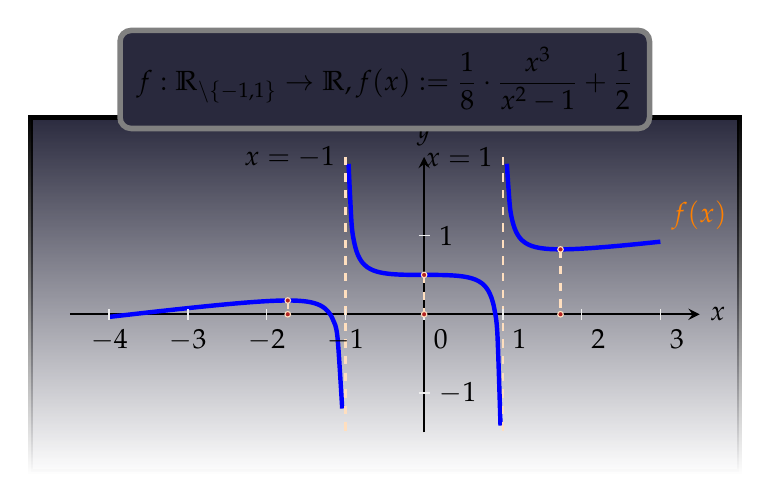
\begin{tikzpicture}
			\filldraw[line width = 2pt, path fading=south, fill=blue!60!yellow!40!black] (-5, -2) rectangle (4, 2.5);
		\draw[thick, -stealth] (-4.5, 0) -- (3.5, 0) node[right] {$x$};
		\draw[thick, -stealth] (0, -1.5) -- (0, 2) node[above] {$y$};
		
		\draw[domain=-4:-1.04, ultra thick, smooth, variable=\x, blue, samples=50] plot ({\x}, {1/8 * (\x*\x*\x)/(\x*\x-1) + .5});
		\draw[domain=-0.96:0.97, ultra thick, smooth, variable=\x, blue, samples=50] plot ({\x}, {1/8 * (\x*\x*\x)/(\x*\x-1) + .5});
		\draw[domain=1.05:3, ultra thick, smooth, variable=\x, blue, samples=50] plot ({\x}, {1/8 * (\x*\x*\x)/(\x*\x-1) + .5}) node[above right, text=orange] {$f(x)$};
		
		\draw[dashed, draw=o1, thick] ($(-1, 0) + (up:2cm)$) node[left] {$x = -1$} -- ($(-1, 0) + (down:1.5cm)$);
		\draw[dashed, draw=o1, thick] ($(1, 0) + (up:2cm)$) node[left] {$x = 1$} -- ($(1, 0) + (down:1.5cm)$);
		
		
		\foreach \i in {-4, -3, -2, -1}{
			\coordinate (p) at (\i, 0);
			\coordinate (pd) at ($(p) + (down:2pt)$);
			\coordinate (pu) at ($(p) + (up:2pt)$);
			
			\draw[draw=w, semithick] (pd) -- (pu);
			\node[below] at (pd) {$\i$};
		};		
		\foreach \i in {0, 1, 2, 3}{
			\coordinate (p) at (\i, 0);
			\coordinate (pd) at ($(p) + (down:2pt)$);
			\coordinate (pu) at ($(p) + (up:2pt)$);
			
			\draw[draw=w, semithick] (pd) -- (pu);
			\node[below right] at (pd) {$\i$};
		};
		\foreach \i in {-1, 1}{
			\coordinate (p) at (0, \i);
			\coordinate (pr) at ($(p) + (right:2pt)$);
			\coordinate (pl) at ($(p) + (left:2pt)$);
			
			\draw[draw=w, semithick] (pl) -- (pr);
			\node[right] at (pr) {$\i$};
		};	
		
		\coordinate (d1) at (-1.732, 0.175);
		\coordinate (d2) at (0, 0.5);
		\coordinate (d3) at (1.732, 0.824);	
		
		\foreach \i in {1, 2, 3}{
			\coordinate (xd\i) at (d\i |- 0, 0);
			
			\draw[draw=o1, dashed, thick] (d\i) -- (xd\i);
			\filldraw[draw=o1, fill=firebrick] (xd\i) circle (1pt);
			\filldraw[draw=o1, fill=firebrick] (d\i) circle (1pt);	
		};
		
		\node[shape=rectangle, line width=2pt, rounded corners, draw=gray, fill = blue!60!yellow!40!black, above=-5pt, inner sep=6pt] at (-0.5, 2.5)	{$f:\mathbb{R}_{\setminus\{-1, 1\}}\to\mathbb{R}, f(x) := \dfrac{1}{8}\cdot\dfrac{x^3}{x^2 - 1} + \dfrac{1}{2}$};
		\end{tikzpicture}

\end{document}